\documentclass[10pt]{article}         %% What type of document you're writing.
\usepackage{graphicx}
\usepackage{hyperref}
\usepackage[dvipsnames]{xcolor}

%%%%% Preamble

%% Packages to use

\usepackage{amsmath,amsfonts,amssymb}   %% AMS mathematics macros

%% Title Information.

\title{Life Goals Data Model}
\author{Adolfo Centeno}
%% \date{2 July 2004}           %% By default, LaTeX uses the current date

%%%%% The Document

\begin{document}

\maketitle

\begin{abstract}
This document implements the Life Goals Data Model.
\end{abstract}

\section{Data Model Desciption}


\textcolor{red}{Metas} personales ( \textcolor{green}{descripcion} )



\section{E-R Model}

Life Goals...

\begin{figure}[h]
     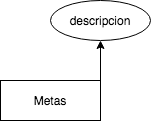
\includegraphics[scale=0.6]{er_lifegoals}
     \caption{Life Goals E-R Model}
\end{figure}
   
\section{Relational Model}
Life Goals Relational Model

\begin{figure}[h]
     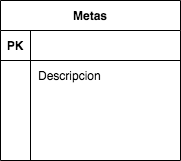
\includegraphics[scale=0.4]{relational_lifegoals}
     \caption{Life Goals Relational Model}
\end{figure}


\section{Build Database in postgresql}

\begin{enumerate}

	\item
	   ssh -i adsoft adsoft@104.198.244.0
	\item
	   sudo -u postgres createdb adsoft-lifegoals;
	\item
	   sudo -u postgres psql;	
    \item 
       list;	   
	\item
	   connect adsoft-lifegoals;
	\item
	   dt
	\item
	   create table metas(descripcion varchar(100));
	\item
	   select * from metas;
	\item
	   insert into metas(descripcion) values ('be like iron man');
	\item
	   update metas set descripcion='go to moon' where descripcion='be hacker';
	\item
	   delete from metas where descripcion=' be like the mexian ellon musk';

	 
	        
   
    	
\end{enumerate}


\end{document}

